\documentclass[12pt,twoside]{article}
\usepackage{amsmath, amssymb}
\usepackage{amsmath}
\usepackage[active]{srcltx}
\usepackage{amssymb}
\usepackage{amscd}
\usepackage{makeidx}
\usepackage{amsthm}
\usepackage{algpseudocode}
\usepackage{algorithm}
\usepackage{graphicx}
\usepackage[spanish, es-tabla]{babel}
\usepackage{multirow}
\renewcommand{\baselinestretch}{1}
\graphicspath{{images/}}
\setcounter{page}{1}
\setlength{\textheight}{21.6cm}
\setlength{\textwidth}{14cm}
\setlength{\oddsidemargin}{1cm}
\setlength{\evensidemargin}{1cm}
\pagestyle{myheadings}
\thispagestyle{empty}
\markboth{\small{Pr\'actica 6. Alan, Josu\'e}}{\small{.}}
\date{}
\begin{document}
\centerline{\bf An\'alisis de Algoritmos, Sem: 2020-1, 3CV2, Pr\'actica 6, 2 de octubre}
\centerline{}
\centerline{}
\begin{center}
\Large{\textsc{Pr\'actica 6: Problema del m\'aximo subarreglo}}
\end{center}
\centerline{\bf{Alan Romero Lucero, Josu\'e David Hern\'andez Ram\'irez}}
\centerline{}
\centerline{Escuela Superior de C\'omputo}
\centerline{Instituto Polit\'ecnico Nacional, M\'exico}
\centerline{$alanrl.escom@gmail.com, josuehernandezr082@gmail.com$}
\newtheorem{Theorem}{\quad Theorem}[section]
\newtheorem{Definition}[Theorem]{\quad Definition}
\newtheorem{Corollary}[Theorem]{\quad Corollary}
\newtheorem{Lemma}[Theorem]{\quad Lemma}
\newtheorem{Example}[Theorem]{\quad Example}
\bigskip
\textbf{Resumen:} La presente pr\'actica desarrolla la soluci\'on del problema del m\'aximo subarreglo con dos algoritmos diferentes: m\'aximo subarreglo mediante recurrencia y un algoritmo de m\'aximo subarreglo cruzado, y m\'aximo subarreglo por fuerza bruta.{\bf Palabras Clave:} {\textit{arreglo, m\'aximo subarreglo, fuerza bruta}}
\section{Introducci\'on}
Cuando se manejan arreglos normalmente se presentan problemas que resultan en un gran reto, tanto para encontrarles soluci\'on como para mejorar el algoritmo que los solucione y no tener soluciones de una complejidad muy alta que terminan siendo inviables. Uno de estos problemas que resulta com\'un o conocido es \textit{el problema del m\'aximo subarreglo}. Este problema puede ser resuelto de muchas maneras, como casi cualquier problema, sin embargo es importante analizar estas soluciones debido a que su complejidad puede aumentar considerablemente, por lo que se analizar\'an dos algoritmos diferentes: mediante fuerza bruta y mediante un algoritmo de m\'aximo subarreglo cruzado.
\section{Conceptos B\'asicos}
El \textit{problema del m\'aximo subarreglo} busca el subarreglo de elementos consecutivos m\'as grande que adem\'as sume el mayor n\'umero en un arreglo de n\'umeros.
\subsection{M\'aximo subarreglo por recurrencia}
Se puede resolver el problema mediante recurrencia, implementando el algoritmo del m\'aximo subarreglo cruzado, utilizando el concepto de divide y venceras para mejorar la complejidad del algoritmo. El algoritmo divide al arreglo desde la mitad en una parte derecha e izquierda, adem\'as se busca el \textit{m\'aximo subarreglo cruzado} entre ambas partes, llam\'andose de manera recursiva.
\subsubsection{M\'aximo subarreglo cruzado}
Primero, el algoritmo del m\'aximo subarreglo cruzado, encuentra el m\'aximo subarreglo de un arreglo desde el medio hacia extremo inferior, posteriormente nuevamente desde el medio hacia un extremo superior. De esta manera encuentra el m\'aximo subarreglo que se encuentra mas centrado del arreglo, devolviendo los \'indices superiores e inferiores del subarreglo interno.
\begin{figure}[ht]
    \centering
    \begin{algorithmic}[1]
        \Procedure{Cruzado}{$A = [A_0,\dots,A_n], low, mid, high$}
            \State $maxleft \longleftarrow 0$
            \State $maxright \longleftarrow 0$
            \State $leftsum \longleftarrow -1x10^100$
            \State $rightsum \longleftarrow -1x10^100$
            \State $sum \longleftarrow 0$
            \For{$ i \text{ from } mid \text{ to } low$}
                \State $sum \longleftarrow A[i]$
                \If{$sum > leftsum$}
                    \State $leftsum \longleftarrow sum$
                    \State $maxleft \longleftarrow i$
                \EndIf
            \EndFor
            \State $sum \longleftarrow 0$
            \For{$ i \text{ from } mid \text{ to } high$}
                \State $sum \longleftarrow A[i]$
                \If{$sum > rightsum$}
                    \State $rightsum \longleftarrow sum$
                    \State $maxright \longleftarrow i$
                \EndIf
            \EndFor
            \State \textbf{return} $[maxleft, maxright, leftsum+rightsum]$
        \EndProcedure
    \end{algorithmic}
    \caption{Pseudo-c\'odigo del algoritmo del m\'aximo subarreglo cruzado}
    \label{fig:cross}
\end{figure}
Dicho algoritmo no tiene \textit{for's} anidados, por lo que dichos bloques tiene complejidad $\mathcal{O}(n)$. El resto de los bloques de c\'odigo tienen complejidad lineal, por lo que se toma el mayor. Finalmente, la complejidad del algoritmo del \textit{m\'aximo subarreglo cruzado} es $\mathcal{O}(n)$.
\subsubsection{Algoritmo}
Ahora, el algoritmo que resuelve completamente el problema primero busca el m\'aximo subarreglo del lado izquierdo, despu\'es del derecho y finalmente el cruzado.
\begin{figure}[h]
    \centering
    \begin{algorithmic}[1]
        \Procedure{Maximo}{$A = [A_0,\dots,A_n], low, high$}
            \If{$low = high = 1$}
                \State \textbf{return} $[low, high, A[low]]$
            \Else
                \State $mid \longleftarrow \frac{low+high}{2}$
                \State $[leftlow, lefthigh, leftsum] \longleftarrow \textbf{MAXIMO}(A, low, mid)$
                \State $[rightlow, righthigh, rightsum] \longleftarrow \textbf{MAXIMO}(A, mid, high)$
                \State $[clow, chigh, csum] \longleftarrow \textbf{CRUZADO}(A, low, mid, high)$
                \If{$leftsum >= rightsum \text{ and } leftsum >= csum$}
                    \State \textbf{return} $[leftlow, lefthigh, leftsum]$
                \ElsIf{$rightsum >= leftsum \text{ and } rifhtsum >= csum$}
                    \State \textbf{return} $[rightlow, righthigh, rightsum]$    
                \Else
                    \State \textbf{return} $[clow, chigh, csum]$
                \EndIf
            \EndIf
        \EndProcedure
    \end{algorithmic}
    \caption{Pseudo-c\'odigo del algoritmo del m\'aximo subarreglo}
    \label{fig:maxm}
\end{figure}
El algoritmo de m\'aximo subarreglo por recurrencia tiene una ecuaci\'on de recurrencia.
\[
    T(n) = 
\begin{cases}
    c, & \text{si } n \leq 1 \\
    T(\frac{n}{2}) + T(\frac{n}{2}) + nc, & n > 1
\end{cases}
\][h]
Reescribiendose con $k = \log_2(n)$.
\[
    T(n) = 
\begin{cases}
    c, & \text{si } k = 0 \\
    T(2\textsuperscript{k-1}) + nc, & n > 1
\end{cases}
\][h]
Resolviendo
\begin{figure}[h]
    \centering
    \begin{equation}
        T(2\textsuperscript{k}) = 2T(2\textsuperscript{k-1}) + nc
    \end{equation}
    \begin{equation}
        \dots 2(2T(2\textsuperscript{k-2})) + 2nc
    \end{equation}
    \begin{equation}
        \text{\textit{i-\'esimo elemento}} \longrightarrow 2^iT(2\textsuperscript{k-i}) + inc
    \end{equation}
    \begin{equation}
        k - i = 0 \longleftarrow k = i
    \end{equation}
    \begin{equation}
        \dots = 2^kT(0) + knc
    \end{equation}
    \begin{equation}
        \dots = 2^kc + knc
    \end{equation}
    \begin{equation}
        \text{Sustituyendo k }\dots
    \end{equation}
    \begin{equation}
        \dots = 2^{\log_2{n}} c + (\log_2{n})nc
    \end{equation}
    \begin{equation}
        \dots = nc + cn\log_2{n}
    \end{equation}
    \caption{Soluci\'on de la ecuacion de recurrencia}
    \label{eq:eq_rec}
\end{figure}
Por lo tanto, la complejidad del algoritmo de m\'aximo subarreglo es $\mathcal{O}(n\log_2{n})$
\newpage
\vfill
\clearpage

\subsection{M\'aximo subarreglo por fuerza bruta}
La soluci\'on del m\'aximo subarreglo mediante fuerza bruta es m\'as directo para su solucion.
\begin{figure}[h]
    \centering
    \begin{algorithmic}
        \Procedure{FuerzaBruta}{$A = [A_0, \dots, A_n]$}
            \State $sumas \longleftarrow [0]$
            \For{ i $\text{ from } 0 \text{ to } n$}
                \State $sumas \text{ \textbf{append} } sumas[ i - 1] + A[i]$
            \EndFor
            \State $maxsum \longleftarrow -1x10^100$
            \State $leftindex \longleftarrow -1$
            \State $rightindex \longleftarrow -1$
            \For{ i $\text{ from } 0 \text{ to } n$}
                \For{ j $\text{ from } 0 \text{ to } n$}
                    \If{$sumas[j+1] - sumas[i] > maxsum$}
                        \State $maxsum \longleftarrow sumas[j-1] - sumas[i]$
                        \State $leftindex \longleftarrow i$
                        \State $rightindex \longleftarrow j$
                    \EndIf
                \EndFor
            \EndFor
            \State \textbf{return} $[leftindex, rightindex, maxsum]$
        \EndProcedure
    \end{algorithmic}
    \caption{Pseudo-c\'odigo del algoritmo mediante fuerza bruta}
    \label{fig:bruta}
\end{figure}

El algoritmo anterior compara todas las posibles combinaciones en el arreglo. Analizando por bloques, se encuentra un primer bloque con un \textit{for} simple, es $\mathcal{O}(n)$, despues se encuentra un bloque \textit{for} con otro bloque \textit{for} dentro, por lo que es $\mathcal{O}(n^2)$. Los demas bloques son de complejidad lineal, por lo que finalmente se toma el mayor. El algoritmo de m\'aximo subarreglo por fuerza bruta es $\mathcal{O}(n^2)$.

\section{Experimentaci\'on y Resultados}
Siempre es bueno asociar la teoría con la pr\'actica, por ende, a continuación se muestran los resultados de la implementaci\'on de estos algoritmos anteriormente descritos.
\begin{figure}
    \centering
    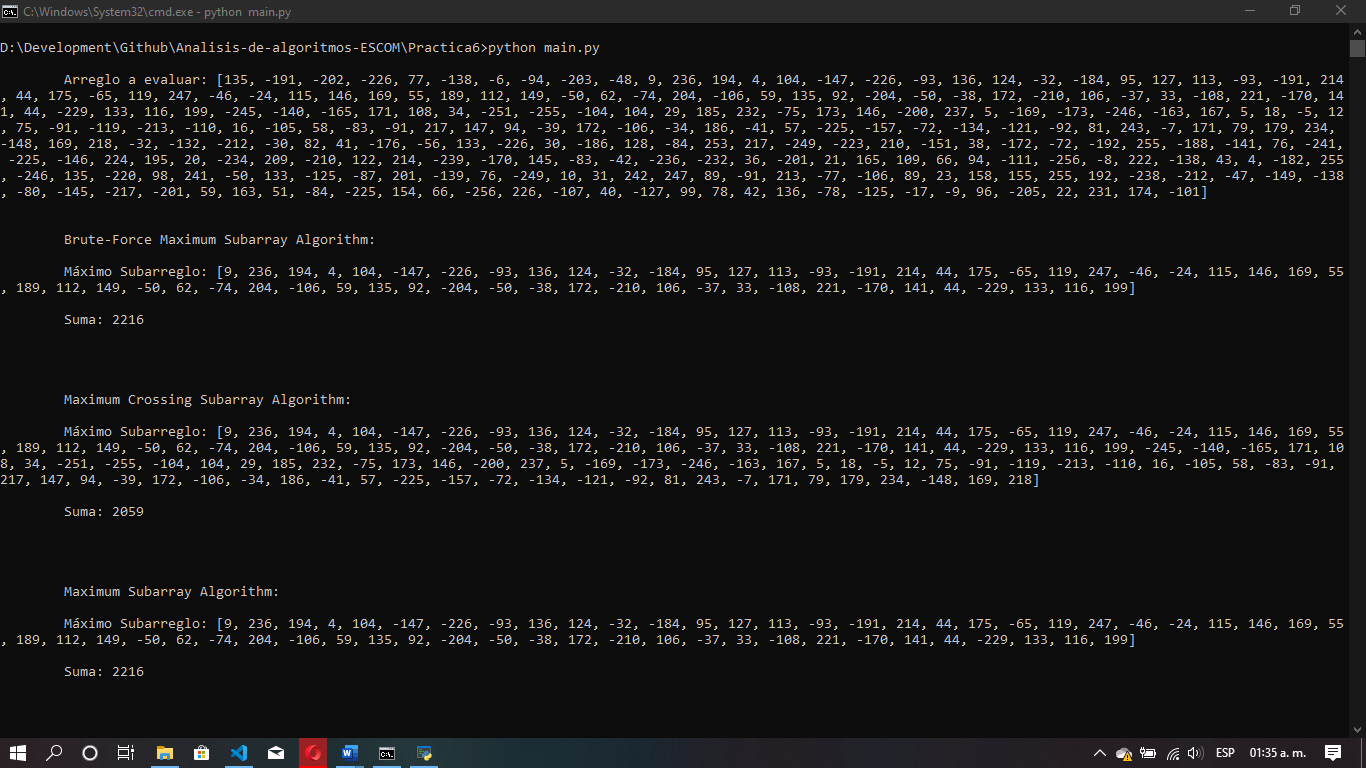
\includegraphics[width=13cm, height=8cm]{console.png}
    \caption{Funcionamiento del algoritmo}
    \label{fig:algoritmo}
\end{figure}

Para tener varios casos de prueba, se implement\'o la autogeneración de los casos de prueba, mediante la generaci\'on de datos aleatorios guardados en una lista, la cu\'al, ser\'a la misma que usaran los tres algoritmos, para que, de este modo, se obtenga una justa comparación.
\newline \newline

\begin{figure}
    \centering
    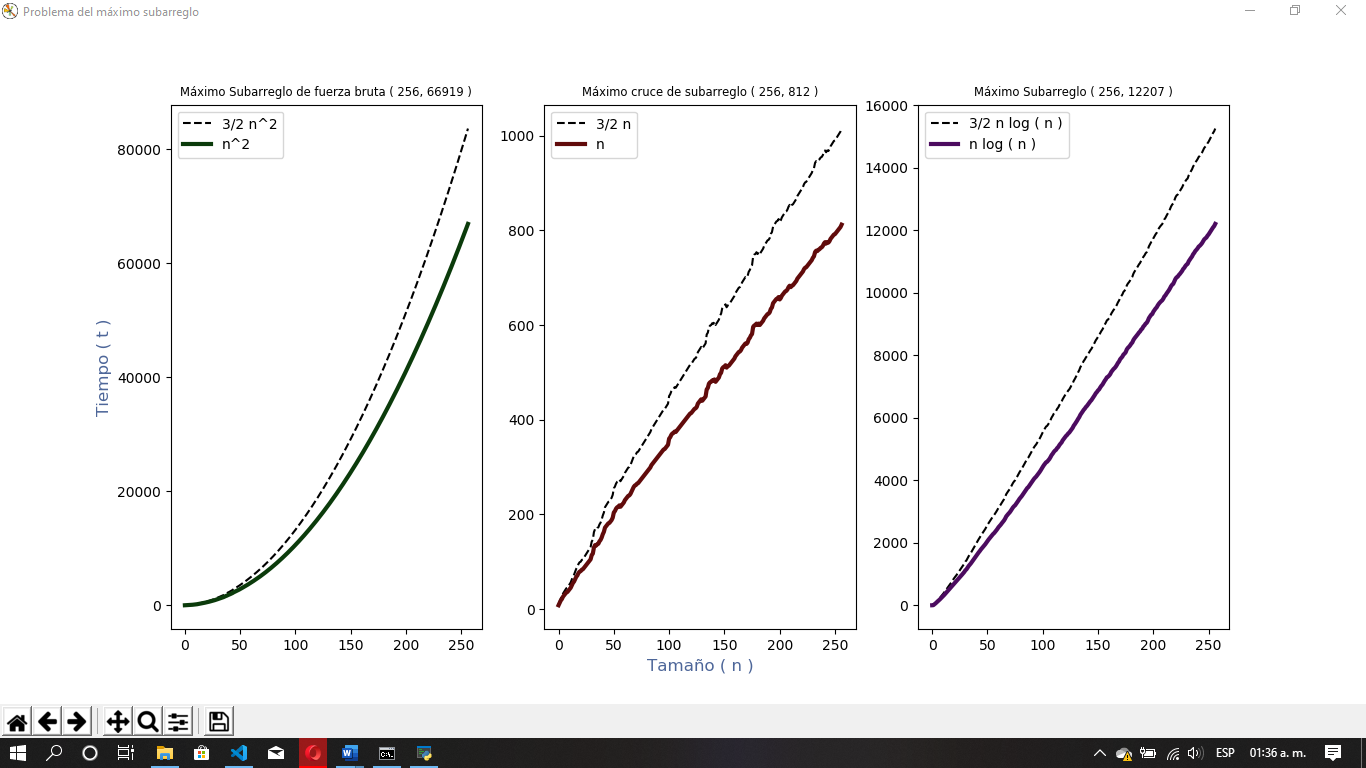
\includegraphics[width=15cm, height=8cm]{result.png}
    \caption{Gr\'aficas de los resultados}
    \label{fig:resultado}
\end{figure}
Con la figura \ref{fig:resultado}, notamos las diferencias en los tiempos que tiene cada implementación de cada algoritmo, lo que conlleva a que su complejidad varía, siendo la m\'as \'optima y estable usandose en las configuraciones de recurrencia. Por otro lado usando el m\'etodo cruzado, var\'ia un poco su estabilidad y con ello su complejidad pasa a ser lineal.
Por \'ultimo usando la fuerza bruta, que es el m\'etodo m\'as corto de implementar, notamos que sacrificamos la complejidad, siendo esta mas alta.
\section{Conclusiones}

\textit{Alan Romero Lucero}. Una vez m\'as se puede ver por que \textit{divide y venceras} es tan importante. La complejidad varia mucho en este caso dependiendo del algoritmo que se utilice. Evidentemente es claro que un problema no debe hacerse por fuerza bruta, y la complejidad de dicho algoritmo es una clara muestra de esa afirmaci\'on. El algoritmo de recurrencia es m\'as interesante para implementar y aun as\'i seguramente habr\'a una implementaci\'on mejor del algoritmo, o una variaci\'on para mejorar su complejidad.

\textit{Josu\'e David Hern\'andez Ram\'irez}.
Como hemos podido notar, el hecho de ahorrar tiempo en la implementaci\'on de un algoritmo, sacrificamos su complejidad, siendo as\'i, que esta aumenta y con ello el tiempo y el consumo de recursos. \newline
Para esto, siempre es recomendable dividir el problema para poder vencer y eso es lo que hace al implementar la recurrencia en este algoritmo, haciendo que su complejidad sea la m\'inima y por ende, el consumo de recursos y de tiempo es mucho menor.
\section{Anexo}
¿Qu\´e retorna la funci\'on de m\´aximo subarreglo cuando todos los valores del arreglo son valores enteros negativos?.
\newline \newline
Si la matriz contiene todos los números no positivas, entonces la solución es el número de la matriz con el valor absoluto más pequeño (o la submatriz vacía, si está permitido).
\section{Bibliograf\'ia}
"Problema máxima subarreglo - Maximum subarray problem - qwertyu.wiki",\newline Es.qwertyu.wiki, 2019. [Online]. Available: \newline https://es.qwertyu.wiki/wiki/Maximum_subarray_problem. [Accessed: 03- Oct- 2019].

\end{document}